\subsection{ArUco marker}
Un marcatore ArUco \cite{ArUco} è un marcatore quadrato sintetico composto da un ampio bordo nero e da una matrice binaria interna che ne determina l'identificatore.\\ 
\`E importante notare che l'identificatore del marcatore non si ottiene convertendo la codifica binaria in un numero a base decimale. Ciò non è possibile poiché per dimensioni elevate dei marcatori il numero di bit è troppo elevato e gestire numeri così grandi non è pratico. Invece, un identificatore marcatore è semplicemente l'indice del marcatore all'interno del dizionario a cui appartiene.
Il bordo nero ne facilita il rapido rilevamento nell'immagine e la codifica binaria ne consente l'identificazione, l'applicazione di tecniche di rilevamento e la correzione degli errori. La dimensione del marcatore determina la dimensione della matrice interna, ad esempio un marker di dimensione 6x6 è composto da 36 bit.\\
I markers vengono raggruppati in set, chiamati dizionari, in funzione della dimensione che determina anche la grandezza della matrice interna. 
Un marker può essere trovato ruotato nell'ambiente, tuttavia è necessario che il processo di rilevamento sia in grado di determinare la sua rotazione originaria, in modo che ogni angolo venga identificato in modo inequivocabile.\\
I marcatori ArUco sono progettati con un algoritmo che può essere matematicamente dimostrato per ottimizzare la distanza tra i marcatori, il che significa che riduce al minimo la possibilità di identificare erroneamente un marcatore per un altro se uno o pochi bit non vengono riconosciuti correttamente.\\
Una volta acquisita l’immagine contenente uno o più markers, il processo di detection viene effettuato tramite 2 step principali. \\
Nel primo step si effettua una detection cercando di trovare, all’interno dell’immagine, delle forme quadrate candidate ad essere possibili markers.\\ 
Nel secondo step è necessario prima trovare gli angoli del marcatore, correggere la distorsione prospettica per ottenere un'immagine che sembri come se il marcatore fosse visto dall'alto, dividere l'immagine risultante in una griglia e confrontare questa griglia di celle bianche e nere con il dizionario fornito per scoprire se esiste una corrispondenza.
\\
\\
\begin{figure} [H]
    \centering
    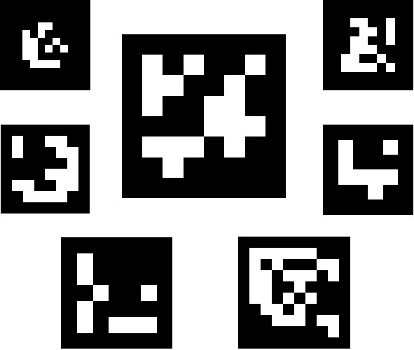
\includegraphics[width=0.5\linewidth]{img/ArUco.jpeg}
    \caption{Esempio di marcatori ArUco}
    \label{fig:ArUco}
\end{figure}

\subsection{ROS2}
Robot Operating System (ROS)\cite{ROS2} \cite{RobOpeSys} è un framework mediante il quale è possibile creare applicazioni robotiche scalabili per robot. Lo scopo di ROS è scomporre il software complesso in parti più piccole e più gestibili, semplificando il processo di sviluppo in quanto fornisce un'interfaccia unificata per la comunicazione tra diversi processi su cui possono essere eseguiti diversi componenti software del robot.\\ 
Inoltre, ROS dispone di un ampio ecosistema di pacchetti di sensori, controllo e algoritmi.\\
ROS ha anche un concetto chiamato server dei parametri, sul quale i parametri globali possono essere memorizzati e accessibili da tutti i nodi. \\
Un nodo non è altro che un file eseguibile all'interno di un ROS package. I nodi del ROS usano una libreria del ROS client per comunicare con altri nodi. I nodi possono pubblicare o iscriversi a un Topic. 
Il nodo è importante un'unità organizzativa che consente a un utente di ragionare su a sistema complesso. L'architettura anonima publish-subscribe consente una comunicazione many-to-many. Uno sviluppatore può osservare eventuali messaggi che passano su un topic creando una sottoscrizione a quell'argomento senza alcuna modifica.
Per governare la comunicazione è necessario stabilire le specifiche dell'interfaccia. Questi messaggi definiscono la
semantica dei dati scambiati. I messaggi definiti vengono comunicati
tra i componenti in modo asincrono, creando un sistema basato sugli eventi. Con questo approccio, un'applicazione può
lavorare nei molteplici domini temporali che derivano dalla combinazione di dispositivi fisici con una serie di componenti software;
ognuno dei quali può avere una propria frequenza di erogazione
dati, accettare comandi o segnalare eventi.

 \subsection{Artificial Potential Field} \label{APF}
Il metodo dei Campi Potenziali Artificiali (o in inglese "Artificial Potential Field", da cui l'acronimo APF), presentato per la prima volta in \cite{khatibAPF}, è un 
metodo per la pianificazione del moto. Si considera il robot come una particella che si muove in un campo potenziale artificiale, il quale è a sua volta la somma di due 
campi: un campo attrattivo (che attrae il robot verso il goal) e un campo repulsivo (che allontana il robot dagli ostacoli). \\
Quindi, data la configurazione del robot $\boldsymbol{q}$, il campo totale è dato da 
\begin{equation}
  J(\boldsymbol{q}) = k_a J_{att}(\boldsymbol{q}) + k_r J_{rep}(\boldsymbol{q}), \: k_a > 0, \: k_r > 0
\end{equation}
e la direzione che il robot dovrà prendere (quindi la "forza" agente sul robot) è data da 
\begin{equation}
  -\frac{\partial  J(\boldsymbol{q})}{\partial \boldsymbol{q}} = -  k_a \frac{\partial  J_{att}(\boldsymbol{q})}{\partial \boldsymbol{q}} - k_r \frac{\partial  J_{rep}(\boldsymbol{q})}{\partial \boldsymbol{q}}
\end{equation}
Per la scelta dei campi attrattivi e repulsivi si può fare rifermiento a \cite{libroRobotica}. Nel nostro caso è stato scelto un potenziale attrattivo Huber-like: 
\begin{equation}
  \begin{cases}
    \frac{1}{2} || \boldsymbol{q} - \boldsymbol{q_G}||^2 \: \: \:  \: \: \: & se \: || \boldsymbol{q} - \boldsymbol{q_G}|| \leq \delta \\
    \delta || \boldsymbol{q} - \boldsymbol{q_G}|| - \frac{1}{2}\delta^2 \: \: \: & altrimenti
  \end{cases} 
  \Rightarrow \boldsymbol{f_{attr}} = 
  \begin{cases}
   \boldsymbol{q} - \boldsymbol{q_G}\: \: \:  & se \: || \boldsymbol{q} - \boldsymbol{q_G}|| \leq \delta \\
    \frac{ \boldsymbol{q} - \boldsymbol{q_G}}{|| \boldsymbol{q} - \boldsymbol{q_G}||}  \: \: \: & altrimenti
  \end{cases} 
\end{equation}
dove con $  \boldsymbol{q_G} $ si indica la configurazione obbiettivo e con $ \delta  $ la distanza di switch tra un potenziale e l'altro. 
Per il campo repulsivo dell'ostacolo $i$-esimo, invece è stato scelto
\begin{equation}
  \begin{cases}
    \frac{1}{\gamma} (\frac{a}{d( \boldsymbol{q},  \boldsymbol{q_{obs_i})}} - \frac{1}{\delta_0})^\gamma \: \: \:  & se \: d( \boldsymbol{q},  \boldsymbol{q_{obs_i}}) \leq \delta_0 \\
    0  \: \: \:  & altrimenti
  \end{cases} 
\end{equation}
%\begin{equation}
% \begin{cases}
%    \frac{1}{\gamma} (\frac{a}{d( \boldsymbol{q},  %\boldsymbol{q_{obs_i}}} - \frac{1}{\delta_0})^\gamma \: \: \:  % & se \: d( \boldsymbol{q},  \boldsymbol{q_{obs_i}}) \leq %\delta_0 \\
%    0  \: \: \:  & altrimenti
%  \end{cases}  \\
%  \Rightarrow \boldsymbol{f_{rep}} = 
%  \begin{cases}
  
%  \begin{split}
%   \frac{1}{d( \boldsymbol{q},  \boldsymbol{q_{obs_i}} )^2} ( \frac{1}{d( \boldsymbol{q},  \boldsymbol{q_{obs_i}}} - \frac{1}{\delta_0})^{\gamma -1}& \nabla d( \boldsymbol{q},  \boldsymbol{q_{obs_i}} ) \\   \: \: \: & se \:  d( \boldsymbol{q},  \boldsymbol{q_{obs_i}} ) \leq \delta_0 
%   \end{split} \\
%    \frac{ \boldsymbol{q} - \boldsymbol{q_G}}{|| \boldsymbol{q} - \boldsymbol{q_G}||}  \: \: \: altrimenti
%  \end{cases} 
%\end{equation}

\begin{equation*}
\Rightarrow \boldsymbol{f_{rep}} = 
\begin{cases}

  \frac{1}{d( \boldsymbol{q},  \boldsymbol{q_{obs_i}} )^2} ( \frac{1}{d( \boldsymbol{q},  \boldsymbol{q_{obs_i}}} - \frac{1}{\delta_0})^{\gamma -1} \nabla d( \boldsymbol{q},  \boldsymbol{q_{obs_i}} )   \: \: \: & se \: d( \boldsymbol{q},  \boldsymbol{q_{obs_i}} ) \leq \delta_0 
   \\
\frac{ \boldsymbol{q} - \boldsymbol{q_G}}{|| \boldsymbol{q} - \boldsymbol{q_G}||} \: \: \:  & altrimenti
  \end{cases} 
\end{equation*}

con $ \gamma = 2$, $ \boldsymbol{q_{obs_i}} $ la rappresentazione dell'ostacolo nello spazio delle configurazioni, con $ d( \boldsymbol{q},  \boldsymbol{q_{obs_i}}) $ la
distanza tra il robot e l'ostacolo e infine con $ \delta_0 $ la soglia sopra la quale l'ostacolo non esercita nessuna influenza sul robot.
Uno dei vantaggi dell'algoritmo APF è che può essere impiegato per effettuare planning online, quindi senza conoscenza a priori della mappa e delle posizioni (o della 
forma) degli ostacoli. Inoltre, grazie alla soglia sulla distanza degli ostacoli presente nel potenziale repulsivo, è possibile associare un potrenziale ad ogni oggetto rilevato entro tale distanza invece che cercare di ricostruirne la forma.

\subsubsection{LOS APF}
 Al fine di vincolare il veicolo a rimanere in una regione limitata di banda attorno al percorso diretto tra due punti di passaggio consecutivi, il metodo precedente viene quindi modificato utilizzando un approccio di Line Of Sight(LOS) \cite{LOSAPF}. In questo caso il potenziale attrattivo non è più associato al waypoint attuale ma ad un punto LOS.
Il calcolo del punto LOS si basa sull'intersezione tra il cerchio di raggio r, centrato sulla posizione del rover e la linea Dk, dove Dk è la linea retta che unisce le coordinate precedente e quelle attuali. Se esistono due punti di intersezione, il punto LOS viene scelto come soluzione più vicina al punto di passaggio corrente. Se non c'è soluzione (cioè il rover si trova a una distanza maggiore di r dalla linea retta tra il punto di passaggio precedente e quello attuale), il punto LOS viene scelto come proiezione ortogonale della posizione della barca sulla linea.
Poiché il punto LOS, con il suo potenziale associato, giace sempre su Dk, questo potenziale in movimento attirerà il rover verso la linea retta tra i due punti di passaggio e costringerà il veicolo a rimanere in una fascia limitata di larghezza inferiore o uguale a r. 
Il valore del punto LOS viene aggiornato ogni volta che viene eseguito l'algoritmo.
\begin{figure} [H]
    \centering
    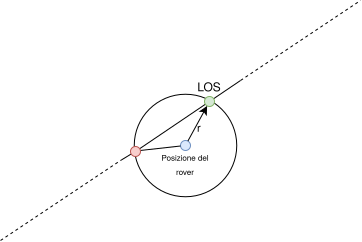
\includegraphics[width=0.5\linewidth]{img/LOSAPFDisegno.png}
    \caption{Tecnica di intersezione}
    \label{fig:LOS}
\end{figure}

\subsection{Sliding Mode Control} \label{SMC_Theory}
Lo Sliding Mode Control (SMC) \cite{algoSMC} è una strategia ad anello chiuso che rientra nella famiglia dei controlli robusti. L'obiettivo è far inseguire al sistema una traiettoria desiderata nello spazio degli stati. Il modello dinamico è noto con certi livelli di incertezza anch'essi noti:
\begin{itemize}
    \item è disponibile un modello $\hat{f}(\boldsymbol {x})$;
    \item è disponibile un modello $\hat{b}(\boldsymbol {x})$.
\end{itemize}
L'incertezza su f è di tipo additivo tale per cui:
\begin{equation}
|f(\boldsymbol {x})-\hat{f}(\boldsymbol {x})|\leq F(\boldsymbol {x})
\end{equation}
con $F(\boldsymbol {x})$ nota. \\
L'incertezza su b è tale per cui:
\begin{equation}
\frac{1}{\beta} \leq \frac{b}{\hat{b}}\leq \beta
\end{equation}
con $\beta$ >1.
\\
Nell'SMC per raggiungere l'obiettivo viene definita una Sliding Surface (SS) definita nello spazio di stato, la quale ha la proprietà di far tendere la dinamica dell'errore a zero. \\ Il sistema di controllo genera l'input di controllo u in modo che:
\begin{itemize}
    \item se il sistema non è sull'SS ci viene portato in un tempo finito;
    \item una volta che il sistema è sull'SS ce lo tiene nonostante le incertezze sul modello.
\end{itemize}
Esistono varie tipologie di SS, dalla letteratura definiamo per esempio $S(t)=s=0$, con s variabile di sliding. La variabile di sliding è una combinazione lineare degli stati errore del sistema ed è definita come:
\begin{equation}
s:=(\frac{d}{dt}+\lambda)^{n-1}\Tilde{\boldsymbol {x}}
\end{equation}
con $\Tilde{\boldsymbol {x}}:=\boldsymbol {x}-\boldsymbol {x_d}$ e $\lambda>0$.
\\
L'input di controllo u è definito come: $u:=\hat{u}+u_{disc}$ dove $\hat{u}$ è una parte model based mentre $u_{disc}$ serve per dare robustezza. \\
Per definire $\hat{u}$ si sfrutta la condizione di permanenza del sistema sulla SS, \\$\dot{s}=\boldsymbol {x}^{(n)}-r^n=0$, da cui con l'ipotesi di modello esatto si ricava $\hat{u}$ come:
\begin{equation}
\hat{u}=\frac{1}{\hat{b}(\boldsymbol {x})}(-\hat{f}(\boldsymbol {x})+r^n)
\end{equation}
Tale termine non ci assicura però nè che la SS venga raggiunta nè che si abbia la permanenza sull'SS in condizioni reali.\\
Per tale motivo si definisce la condizione di sliding $s\dot{s}\leq -\eta|s|$ la quale ci assicura il raggiungimento della SS in un tempo finito. Dalla sliding condition dobbiamo poi sintetizzare $u_{disc}$, quindi scegliendo dalla letteratura:
\begin{equation}
u_{disc}=-\frac{K}{\hat{b}}sgn(s)
\end{equation}
dobbiamo ricavare K in modo che soddisfi la condizione di sliding.
\\
Nel caso in cui il modello sia incerto sia su f che su b si definisce k come:
\begin{equation}
K\geq \beta \{\eta+F(\boldsymbol {x})+(\beta-1)|\hat{f}(\boldsymbol {x})-r^n|\}
\end{equation}
\subsection{Controllori PID}
    \begin{figure}[h]
      \centering
      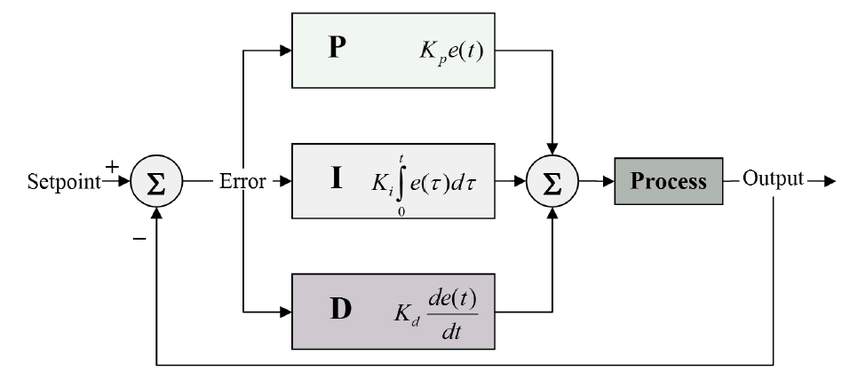
\includegraphics[width=0.8\textwidth]{img/PID.png}
      \caption{Rappresentazione a blocchi di un controllore PID}
      \label{img:PID}
    \end{figure}
  Si consideri un generico sistema $P(s)$ da controllare attraverso un controllore $C(s)$, come mostrato in \autoref{img:PID}. Esistono varie tecniche per realizzare il controllore; una delle più utilizzate è la tecnica PID, dove l'acronimo definisce le tre leggi di controllo Proporzionale, Integrale e Derivativo. L'errore misurato, dato dalla differenza tra il riferimento e l'uscita effettiva 
    del sistema, è l'ingresso del controllore, il quale genera un segnale di uscita $u$ composto dalle tre componenti 
    proporzionale, integrale e derivativa:
    \begin{displaymath}
      \boldsymbol{u} = K_P  \boldsymbol{e}  + K_D  \dot{ \boldsymbol{e}} + K_I \int_{0}^t  \boldsymbol{e}(\tau) d\tau 
    \end{displaymath}
  La funzione di trasferimento del sistema $C_{PID}(s)$ vale quindi 
  \begin{displaymath}
    C_{PID}(s)=K_P + \frac{K_I}{s}+ K_Ds = \frac{K_Ds^2 + K_Ps + K_I}{s}
  \end{displaymath}
  Le azioni dei tre contributi sono le seguenti:
  \begin{itemize}
    \item Il contributo proporzionale permette di migliorare la prontezza della risposta e ridurre l'errore a regime permanente
    \item Il contributo integrale permette eliminare l'errore a regime permanente peggiorando però la risposta transitoria
    \item Il contributo derivativo permette di aumentare la stabilità del sistema.
  \end{itemize}

\subsubsection{Schemi anti wind-up}
Il fenomeno del wind-up è dovuto all’azione integrale. Questo fenomeno si innesca quando i sistemi di attuazione che trasformano il segnale di comando nell’azione di controllo vanno in saturazione. Questo accade quando e(t), che a causa della saturazione  rimane costante in segno, viene integrato.\\
Quando poi cambia il segnale di riferimento, e(t) cambia segno ma prima di osservare una variazione del segnale di comando le componenti integrali del PID si devono scaricare cosi da uscire dalla saturazione. Questo può richiedete tempi lunghi con una conseguente perdita di reattività. \\
Si usano degli schemi anti wind- up per prevenire questo fenomeno. La tecnica anti wind-up più nota in letteratura  è la  "back calculation and tracking". \\
 \begin{figure}[h]
      \centering
      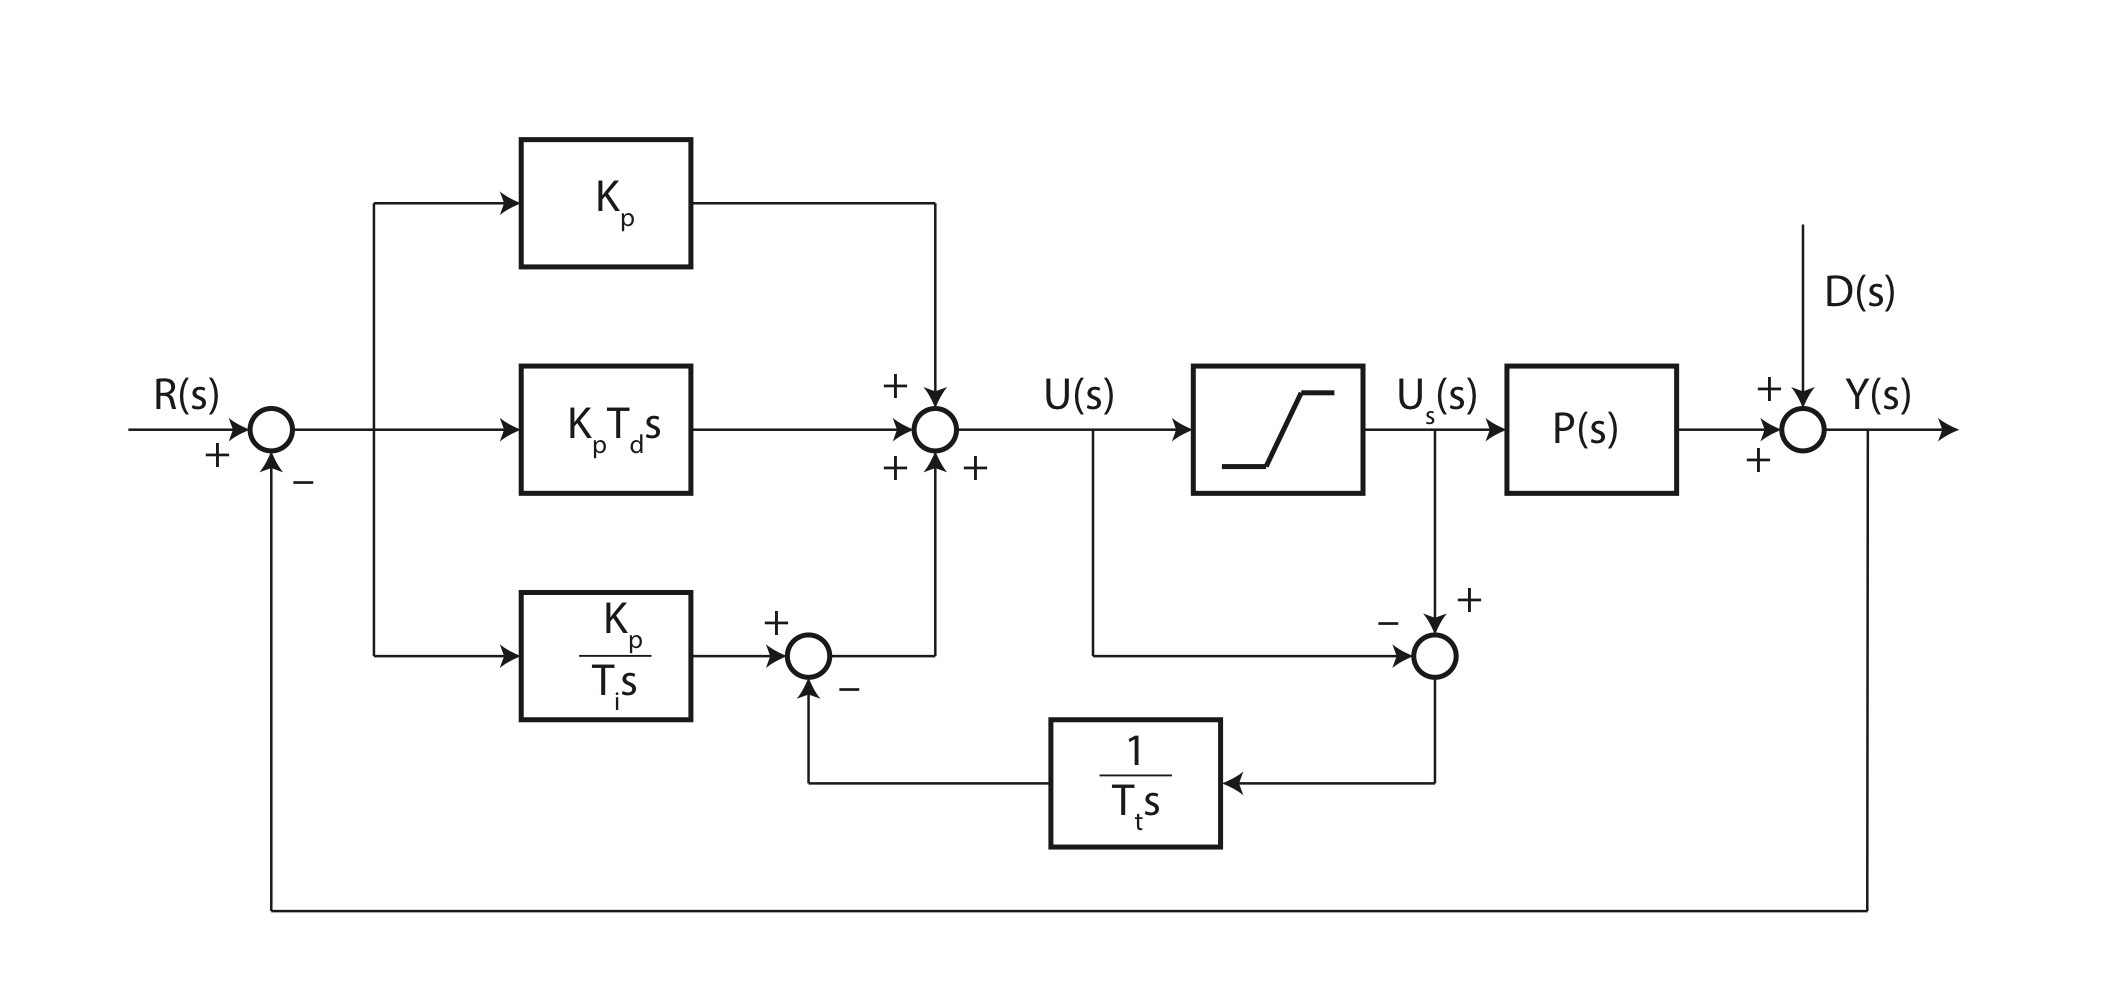
\includegraphics[width=0.8\textwidth]{img/anti wind-up.JPG}
      \caption{schema PID con back calculation and tracking}
      \label{img:antiwindup}
    \end{figure}
In questa tesnica il segnale di comando viene confrontato con l'azione di controllo per capire quando gli attuatori sono in saturazione. Quando il sistema si trova in saturazione si modifica il termine dell'azione integrale per contrastare gli effetti della carica. L'azione integrale viene scaricata attraverso una legge che porta il suo contributo il più possibile vicino al valore di soglia con una certa costante di tempo opportuna.
\begin{equation}
U(s)=\underbrace{U_P(s)+U_D(s)+U_I(s)}_\text{PID ideale}+\underbrace{\frac{1}{T_t}(U_s(s)-U(s)}_\text{BC\&T}
\end{equation}